\label{ref:moaa-exec}

\section{User Input File}
\label{sec:uif}

The creation of a MOAA application starts with the definition of a \gls*{UIF} in \textit{.xml} format.
The UIF contains a set of required and optional settings for MOAA.
The required settings are a list of irradiation cases, a list of decay times, and a list of cells.
Within the irradiation cases, the user must specify an associated MCNP input file, an irradiation time, and an irradiation power.

% Basic user input description
Listing \ref{uif1} displays a minimal MOAA input file which includes a single irradiation case, a single decay time step, and a single cell.
The irradiation case geometry and material definition are specified by the MCNP input file \texttt{test1.i} with an irradiation duration of 1 day and a reactor power of 100 MW.
The irradiation period is followed by a decay of 1 day.
The user-defined cell for the calculations is cell number $1$ of the MCNP input file.
\lstinputlisting[language=xml, caption={Example of a minimalistic MOAA UIF.}, label={uif1}, captionpos=b, xleftmargin=18pt]{./moaa-input-minimal.xml}


\section{ATR case}
\label{sec:ap-atr}

% ATR input file
The required settings within the irradiation cases include an MCNP input file, an irradiation time, an irradiation power divided into five lobe powers: NW, NE, C, SW, SE.
Additionally, the user must provide the F7 tally identification number that will be used for adjusting the lobe powers.

Listing \ref{uif2} displays a typical UIF for an ATR experiment.
This application includes a single irradiation case, two decay times, and 1800 cells (only four are shown).
The irradiation case geometry and material definition are specified by the MCNP input file \texttt{ne71a.i1}, with an irradiation duration of 3 days, and a total reactor power of 120 MW, which is subdivided into five reactor lobes.
The irradiation period is followed by a decay of 12 hours.
The user-defined cells for the calculations are cells number $501101$, $501102$, $508459$, and $508460$ of the MCNP input file.
Finally, the adjusted lobe power calculation relies on tally number $7$.
\lstinputlisting[language=xml, caption={Example of a typical MOAA UIF for an ATR experiment.}, label={uif2}, captionpos=b, xleftmargin=18pt]{./moaa-input-atr.xml}


\section{Executing MOAA}

The execution of MOAA requires the installation of several common dependencies, such as \textit{NumPy} \cite{numpy} and \textit{Pandas} \cite{pandas}.
The recommended installation procedure is to create a Python virtual environment in \texttt{\$MOAA-VENV} for their installation.
The next step is the installation of the MOAA package.

After the installation, the user can choose to execute MOAA either in interactive or batch mode from the command line.
The only required positional argument is the UIF: \texttt{moaa input.xml}.
The environment path must include MCNP and SCALE executables for the successful run of the UIF.
Additionally, the UIF directory must contain a subdirectory holding the MCNP input files defining each irradiation case.
Running MOAA in batch mode uses a submission script for execution on a \gls*{HPC} cluster, as shown in Listing \ref{pbs}.

% PBS Script
\lstinputlisting[language=Bash, caption={HPC job submission script.}, label={pbs}, captionpos=b, xleftmargin=18pt]{./moaa_runner.pbs}

The execution of MOAA may include several optional arguments that give the user greater flexibility.
These arguments include the definition of a non-default output directory, a non-default log-file name, and the choice of different verbosity levels for the logged information.

% ASYNCIO
During the execution of MOAA, the generation and execution of the SCALE input files, as well as the parsing of the SCALE output file, occurs concurrently.
% Definition of concurrent (concurrent != parallel)
% Instead, a process might start, then once it's waiting on a specific instruction to finish, switch to a new task, only to come back once it's no longer waiting.
MOAA relies on the Python standard library \textit{asyncio}, which is the foundation for Python asynchronous frameworks, allowing for the creation and execution of co-routines and an overall reduction in the run times.


\section{Simulation output}
\label{sec:out}

Upon successful execution of a MOAA simulation, a number of files are created in the UIF directory based on the user-defined settings.
The most common files are an execution log-file \textit{MOAA.log} and a \textit{.xlsx} spreadsheet with the isotopic composition.

% Log File
MOAA leverages the Python built-in logging module for informing the user on the progression of the simulation.
The log-file contains all the logging messages produced during the execution, which may include warnings and errors.

% Excel files
The generated spreadsheets contain the isotopic composition at the end of the last irradiation step and after each decay step.
The different tabs of the spreadsheet separate the results by irradiation cell.
% Additional xlsx
The MOAA calculation may produce additional \textit{.xlsx} files containing the simulation results in the user-defined units of interest, such as Curies and Watts.

The choice of \textit{.xlsx} format for the output files comes from the fact that most experiment analysts and clients are familiar with spreadsheet editors.
The results in these files can be easily visualized with the editor's built-in plotting capabilities or with python using \textit{Pandas} and \textit{Matplotlib} \cite{matplotlib}.
An example of such visualization using the isotopic composition of the input file example from Section \ref{sec:uif} is presented in Figure \ref{fig:output-ex}.

% Example output figure
\begin{figure}[htbp!]
  \begin{center}
    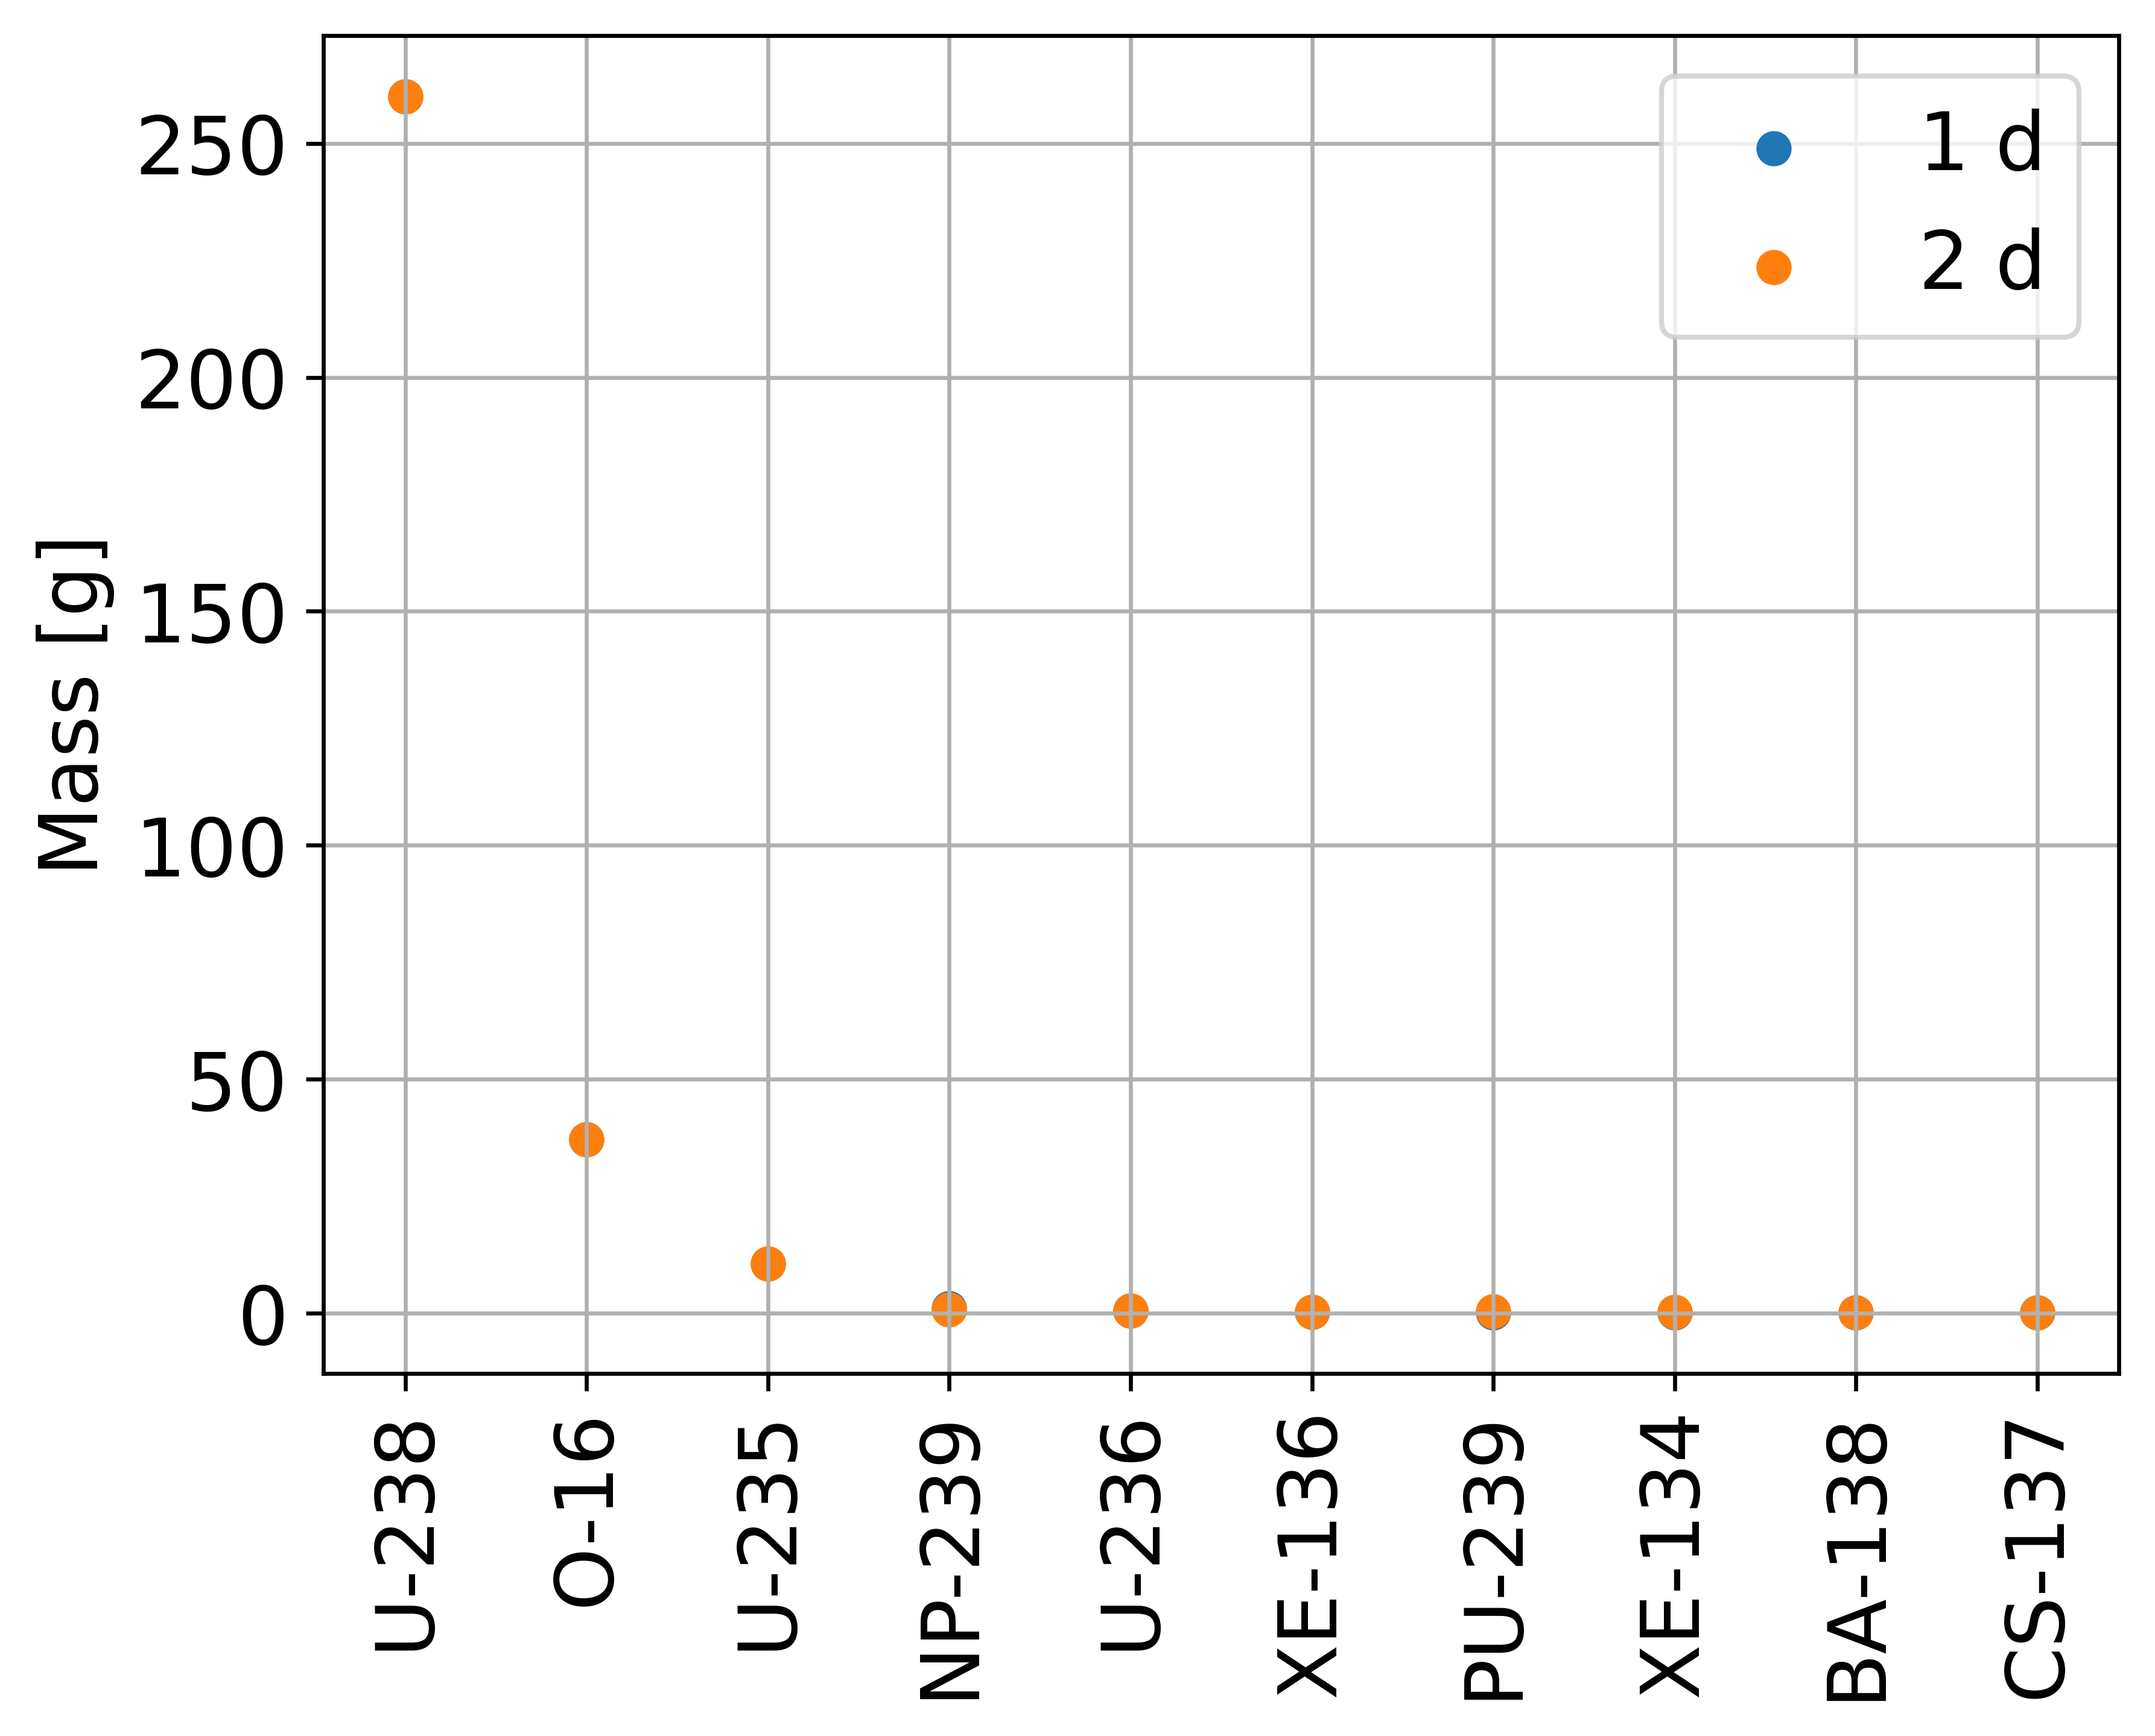
\includegraphics[scale=0.60]{figures/test1_grams}
  \end{center}
  \caption{Example of an output processing with \textit{matplotlib} for an experiment of UO$_2$ after a one day irradiation (in blue) and one day decay (in orange). Only the ten largest contributors to the total mass are displayed.}
  \label{fig:output-ex}
\end{figure}

Furthermore, MOAA has the ability to combine the results for a group of user-defined cells.
When several cells form a region of interest, MOAA combines the source term from all of them.
This feature is helpful in cases wherein an experiment capsule is defined by multiple cells and materials, for example.
This step allows for computing a source term for the whole capsule and thus easing the results post-processing.


% \section{Software structure}

% % Object oriented
% % Advantages of Object-Oriented Programming
% MOAA is a python package that leverages object-oriented programming, in which the code structure is divided into objects that bundle different steps of the calculations.
% This feature gives the code greater modularity which eases the software maintenance and  development.

% This section of the article provides an overview of the code and a brief description of some of the modules integrating MOAA.
% Figure \ref{fig:tree} displays the code structure of MOAA.
% The different modules contain the following:
% \begin{itemize}
% \item \textit{constants.py}: constants necessary for MOAA, such as the Avogadro's number and conversion factors between different units.
% \item \textit{errors.py}: definition of the classes handling the errors in MOAA, such as errors for an invalid UIF or wrong units choice.
% \item \textit{file.py}: definition of a base class for handling and parsing MCNP and SCALE files.
% \item \textit{irradiation\_case.py}: definition of the class \texttt{IrradiationCase} which handles all the information related to the irradiation cases.
% \item \textit{\_\_main\_\_.py}: MOAA main driver. It sets up the execution workflow of MOAA.
% \item \textit{material\_file.py}: definition of the class \texttt{MaterialFile} that parses and produces materials from \textit{.csv} data for MCNP and SCALE.
% \item \textit{moaa.py}: definition of the class \texttt{Moaa} which defines the main calculation workflow.
% \item \textit{moaa\_log.py}: MOAA logging configuration and associated functions.
% \item \textit{nuclide\_data.py}: the nuclide mass data constants necessary for MOAA.
% \item \textit{reaction\_rate.py}: definition of the class \texttt{ReactionRate} which stores minimal data to represent a reaction rate in a cell for a specific material.
% \item \textit{settings.py}: MOAA default settings that can be changed by the user.
% \item \textit{time\_increment.py}: definition of the class \texttt{TimeIncrement} which handles the conversion of time units.
% \item \textit{user\_input.py}: definition of the class \texttt{UserInput} that parses the UIF.
% \item \textit{utils.py}: several functions that support the execution of MOAA, such as the creation of new directories, and the definition of the asynchronous task handler.
% \item \textit{mcnp} and \textit{scale} directories contain the modules that define all the classes associated with the handling of the input and output files of MCNP and SCALE, respectively.
% \end{itemize}

% % Directory tree
% \begin{figure}[htbp!]
%   \begin{center}
%     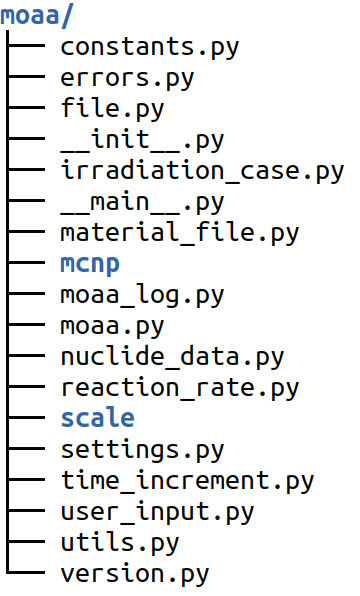
\includegraphics[scale=0.33]{figures/moaa-directory}
%   \end{center}
%   \caption{MOAA directory tree.}
%   \label{fig:tree}
% \end{figure}
